\documentclass[a4paper,11pt]{book}

% Paketi za nas jezik (optimalni)
\usepackage{cmsrb}
\usepackage[OT2,T1]{fontenc}
\usepackage[serbian]{babel}

\usepackage{graphicx}
\usepackage{lmodern}
\usepackage{hyperref}
\usepackage{listings}


\makeatletter
\newenvironment{chapquote}[2][2em]
  {\setlength{\@tempdima}{#1}%
   \def\chapquote@author{#2}%
   \parshape 1 \@tempdima \dimexpr\textwidth-2\@tempdima\relax%
   \itshape}
  {\par\normalfont\hfill--\ \chapquote@author\hspace*{\@tempdima}\par\bigskip}
\makeatother

\title{\Huge \textbf{Modelovanje autonomnog sistema za kompaktan uzgoj biljaka} \\ \huge Modelovanje i simulacije}
\author{\textsc{Aleksandar Stojanović RN97-2018}}


\begin{document}

\maketitle
\tableofcontents

%\mainmatter
\chapter*{Uvod}

\section*{Svrha rada}
Ovaj rad je stvoren sa ciljem da opiše jednostavno i pristupačno rešenje za proizvodnju hrane u veštačkim uslovima.\\

\noindent U ovom radu prezentovaću svoj pristup dizajniranja ovakvog sistema. Detaljno cu analizirati principe rada individualnih podsistema koji sačinjavaju ovu jedinicu i simulirati njihov rad.

\section*{Uzgoj u zastvorenom prostoru}
Ovakav vid proizvodnje sa urbanizacijom postaje sve popularniji. Kako gradovi postaju sve veći, potreba za organskom hranom raste te se ljudi okreću alternativnim metodama uzgoja.\\

Kada je reč o zatvorenim prostorima, u glavnom se misli na kontrolisano okruženje koje ima za cilj da olakša razvoj biljke pa kasnije i samih plodova. Ovo se postiže adekvatnim planiranjem što podrazumeva razmatranje i ispunjavanje svih uslova neophodnih za rast. 

\section*{Tradicionalan ili zatvoren uzgoj}
Dok nam tradicionalan pristup uzgoju olakšava logistiku i nudi dosta pogodnije mogućnosti za ekspanzije, zatvoren pristup pruža kompletno kontrolu nad samim okruženjem. Pored toga biljka je kopletno izolovana od negativnih spoljašnjih faktora kao što su:

\begin{itemize}
  \item paraziti,
  \item naglih oscilacija temperature,
  \item prevelike količine padavina.
\end{itemize}

\noindent Sama činjenica da je biljka u izolovanom okruženju nam omogućava da bliže pratimo njen razvoj. Ovo posebno dolazi do izražaja kod uočavanja problema u ranim fazama kada je jedinka najosetljivija što se tiče uticaja okoline.

Pored otkrivanja problema omogućava nam optimizaciju procesa uzgoja što dovodi do efikasnije proizvodnje. Pod ovim se podrazumeva uzgoj bilja vrhunskog kvaliteta i visokog prinosa u celogodišnjoj proizvodnji bez ograničenja u pogledu sezone ili optimalnih uslova gajenja, kako u atmosferi tako i u zoni ukorenjavanja gajenih biljaka. Precizna, manuelna ili automatska kontrola temperature i relativna vlažnost vazduha, provetravanje, ishrana i navodnjavanje i održavanje idealnog vodnog i vazdušnog režima zemljišta ili supstrata doprinosi eliminisanju ili maksimalnom smanjenju potencijalnog rizika.

\chapter{Priprema}

%\begin{chapquote}{Author's name, \textit{Source of this quote}}
%``This is a quote and I don't know who said this.''
%\end{chapquote}

\section{Definisanje problema}
Dakle, naš cilj je izrada autonomne jedinice koja radi bez čovekovog prisustva. Kako bismo to postigli moramo se osloniti na nekakvu upravljačku jedinicu koja ce biti zadužena za kontrolu celokupnog sistema uz oslonac na senzore. 

Glavna prepreka je limitirana količina prostora koja nam je na raspolaganju. Kada je reč o uzgoju u zatvorenim prostorima podrazumeva se da nam je sam prostor jako važan resurs i potrebno je iskoristiti ga što efikasnije. Tek kada je prostor pravilno iskorišćen možemo započeti izradu ostlaih delova sistema.

Da bismo prostor koristili efektivno bitno je da unapred definišemo funkcionalnosti našeg sistema: 

\hrulefill

1. Merenje i regulacija temperature,

2. Merenje vlažnosti zemlje i ambijenta,

3. Regulacija svetlosnog ciklusa,

4. Regulacija brzine ventilatora,

5. Zalivanje biljke,

6. Logovanje 

\hrulefill

\noindent Imajuci ove funkcije na umu mozemo odrediti grub plan projekta. U sledećoj tački ćemo da detaljo definisati svaku od ovih funkcija i opisati hardver koji ćemo koristiti za izradu. Cilj nam je da hardver zauzme sto manje prostora kako bi ostalo što vise prostora za rad sa biljkom.

\section{Plana izrade projekta}

\subsection{Jedinica}

Sistem će biti smešten u kabinet dimenzija 35x35x60 koji je izradjen od metala. Ova veličina ce podržati biljku srednjih veličina. Neophodno je da unutrašnjost kabineta bude obložena reflektivnim materijalom koji će dobrineti da biljka iskoristi pun potencijal svetla. Pored reflektivnog materijala, unutrašnje ivice sistema je potrebno obložiti gumom kako bismo efektivno izolovali sistem od sredine.

Na vrh(plafon) kabineta neophodno je ugraditi nekakvo rešenje za fiksiranje svetla u vidu kuka. Za kuke se kače sajle koje će držati svetlosnu fiksturu. Na poledjini kabineta izbušićemo dve rupe za kačenje ventilatora koji ce obezbediti cirkulaciju. Donji otvor će služiti za unos svežeg vazduha dok se na gornji fiksira filter vazduha radi kontrole mirisa. Razlog ovoga je sledeći:

Ako pogledamo sledeće slike\footnote{AC infinity je kompanija koja se bavi solucijama za hladjenje, vise na: https://www.acinfinity.com/pages/technical-guides/cabinet-cooling-and-ventilation.html}

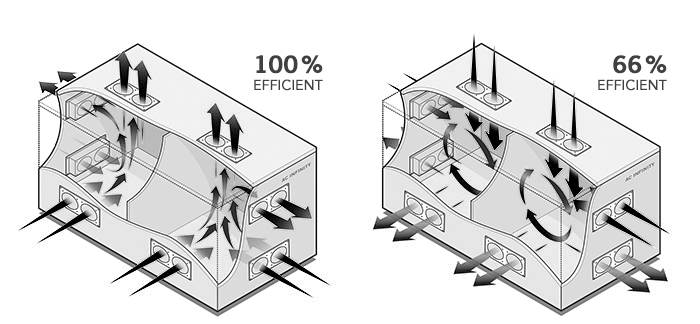
\includegraphics[width=\textwidth]{10060.jpg}
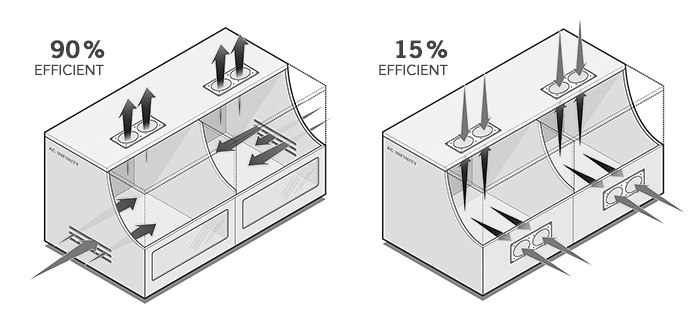
\includegraphics[width=\textwidth]{9015.jpg}

Možemo uvideti da je najbolja konfiguracija ventilatora ona koja vazduh uvlači pri dnu, a topao izbacuje pri vrhu. 

\subsection{Kontroler}
\noindent \\ Što se kontrolera tiče, budući da ovakav sistem zahteva kontinualan rad sto podrazumeva dugoročno opterećenje, Adruino Uno\footnote{Arduino Uno je open-source rešenje u vidu kontrolera za IoT projekte koji pruža mnoštvo mogućnosti. Vise na: https://www.arduino.cc/en/Guide/Introduction} je idealno rešenje jer nudi stabilnost pod dugoročnim radom i jednostavnu integraciju senzora. Pored stabilnosti i male veličine ako pogledamo njegov dijagram možemo uočiti da imamo izlaze od 3.3V i 5V sto je idealno za napajanje senzora i releja.

Kontroler če biti smešten izvan sistema sa spoljašnje strane unutar odeljka zajedno sa protobordom za povezivanje svih komponenti i releja. Ovo će predstavljati mozak sistema odakle ćemo rutirati kablove. Kao odeljak, plastična razvodna kutija je dimenzija 20cm x 20cm x 5cm je sasvim dovoljna za naše potrebe.

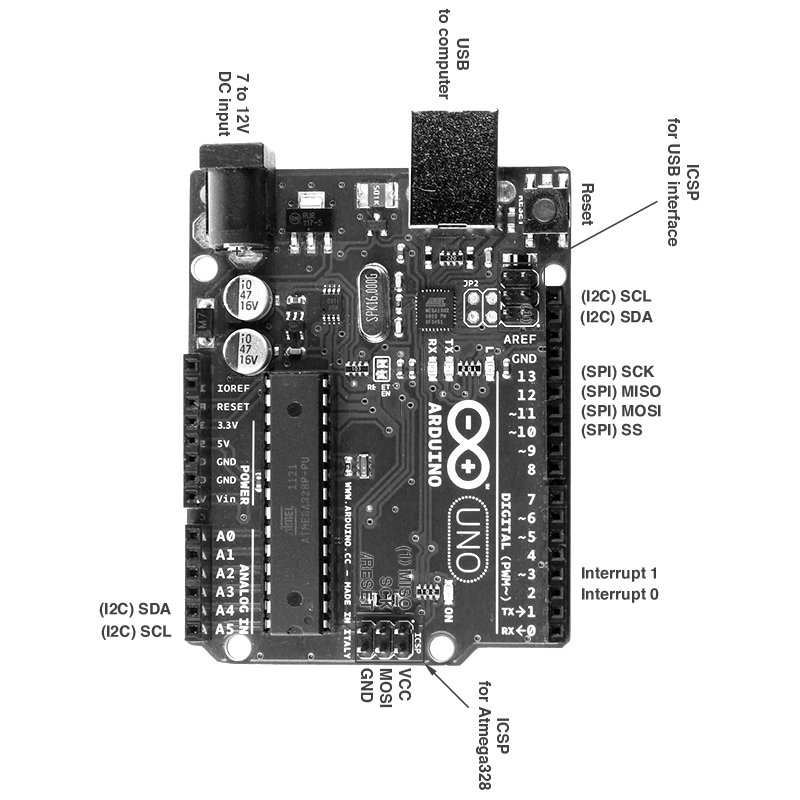
\includegraphics[width=\textwidth]{uno_pinout.png}

\subsection{Monitor}
Kao monitor za feedback sistema koristicemo mali I2C\footnote{I2C protokol služi za serijsku komunikaciju sa mikrokontrolerima. Vise na: https://i2c.info/} OLED ekran 128x32 veličine 0.91 inča kao dugoročno rešenje dok će serijski port biti primarno korišćen u početnim fazama izrade.

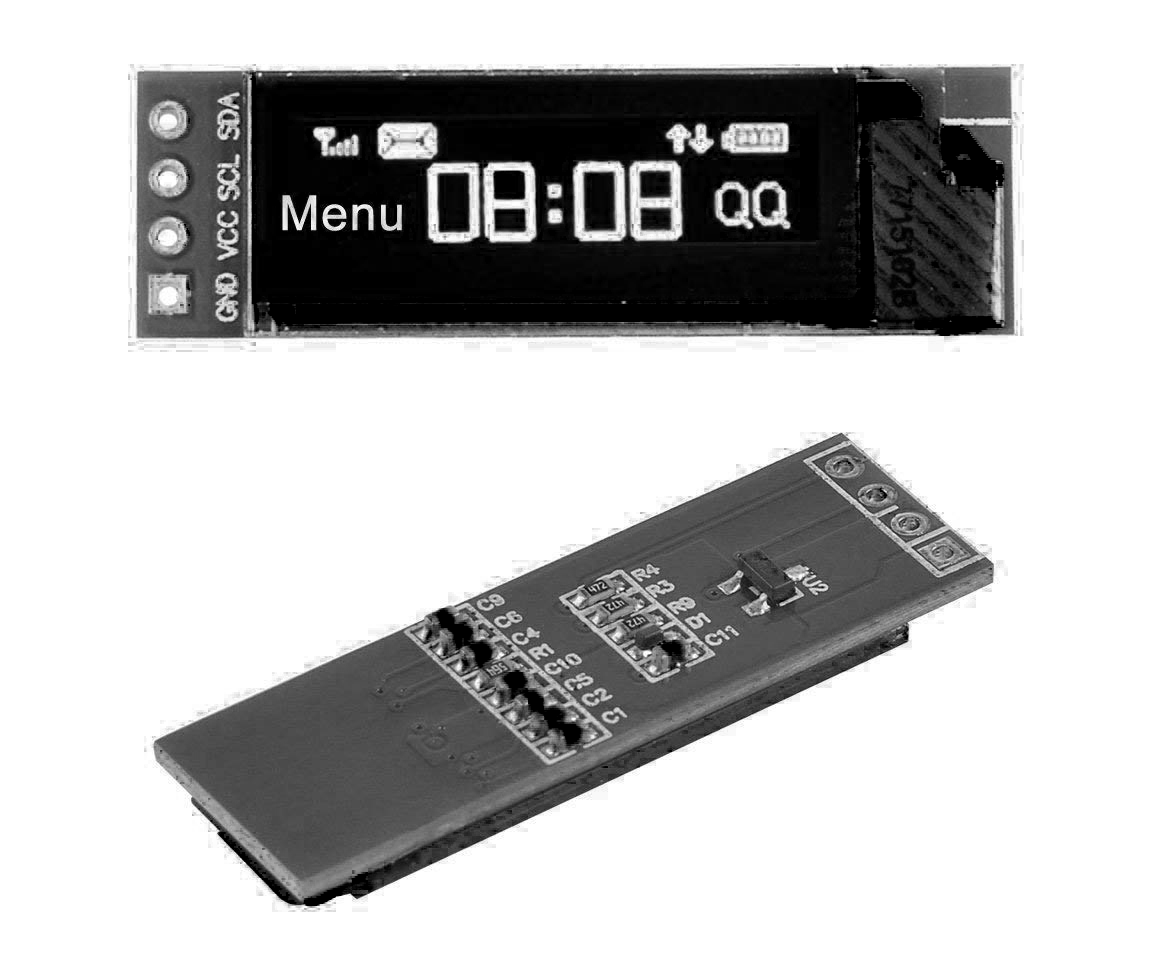
\includegraphics[width=\textwidth]{oled.png}

\subsection{Merenje temperature i regulacija}

Čest problem sa kompaktnim zatvorenim baštama je visoka temperatura.

Merenje temperature je krucijalan korak jer je to jedan od glavnih faktora okruženja. Različite biljke zahtevaju različite uslove poput povećane vlage, stoga neophodno je koristiti adekvatan hardver.\\ 

\noindent DS18B20\footnote{Digitalni senzor toplote koji nudi 9-bit do 12-bit vrednosti toplote izražene u celizijusu. Vise na: https://datasheets.maximintegrated.com/en/ds/DS18B20.pdf} je senzor po izboru iz razloga što je fabrički izolovan, ima dosta širi opseg vrednosti od očekivanog unutar sistema i napaja se sa 3.3V ili 5.5V.

Regulaciju rešavamo korišćenjem ulaznih i izlaznih ventilatora(vise o regulaciji temperature kasnije u radu).

\subsection{Merenje vlažnosti zemlje i ambijenta}
Praćenjem vlažnosti zemlje nam omogućava da automatizovano zalivamo biljku u zavisnosti od njenih potreba. Za razliku od fiksnih ciklusa zalivanja kod kojih može doći do preteranog navodnjavanja ovde se mehanizam za navodnjavanje aktivira samo kada je to potrebno. Ovo sprečava prekomerno zalivanje sto dovodi do raznih problema poput:

\begin{itemize}
  \item Nedostatka kiseonika u zemlji za korenov sistem,
  \item gljivično oboljenje korena,
  \item nedostatak hranjivih materija usled prekomernog ispiranja
\end{itemize}

Za vlagu ambijenta koristimo HR202 senzor vlage u vazduhu, a za zemljiste koristimo kapacitivni senzor LDTR-WG0236.

Ovaj senzor vraća analognu vrednost što znaci da dobijamo kontinualan signal velike preciznosti. 

Ako pogledamo sledeci grafik:

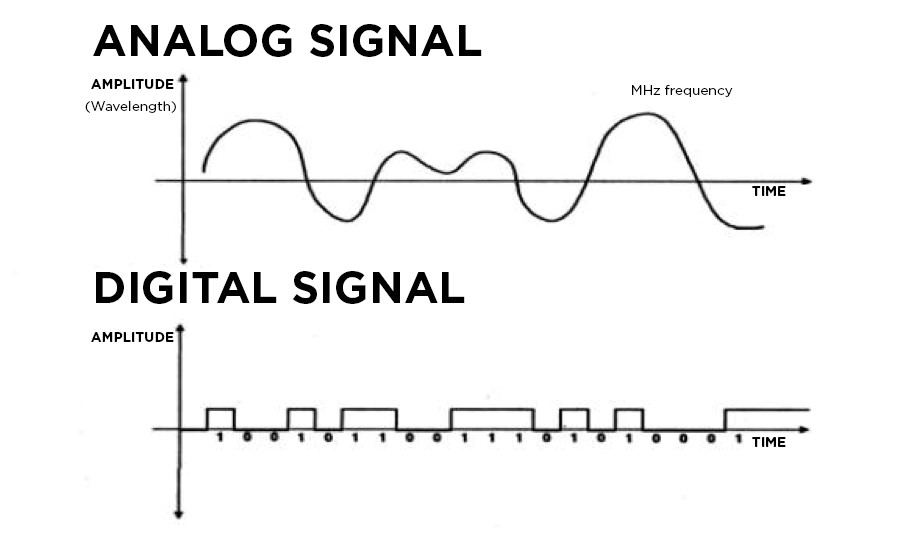
\includegraphics[width=\textwidth]{digital-analog.jpg}

Ovo znači da ćemo uvek dobijati neku vrednost vlage za razliku od digitalnih koji za neku vrednost X vraća 0 ako je izmerena manja ili 1 ako je veća. Tačnu vrednost valge za aktivaciju ćemo utvriditi merenjem.

\subsection{Regulacija rada ventilatora}
Ventilatori nam koriste za razmenu vazduha sa okolinom. Sa druge strane, kako utičemo na njihovu brzinu jedinica će se brže odnosno sporije hladiti.

Da bismo pronašli odgovarajuću veličinu ventilatora za sistem moramo odrediti zapreminu samog prostor sa kojim radimo:

\[ 35cm * 35cm * 60cm =  73500cm^3 = 2.595628ft^3\]

Iz ovoga vidimo da su nam dovoljno obicni 12V ventilatori. Budući da se na izlaz kači filter vazduha koji u sebi sadrži dva 60mm ventilatora koji po specifikaciji pomeraju 38.35cfm a nasa jedinica ima samo ~2.5, na ulaz možemo staviti jedan ventilator od 120mm koji cemo uključivati u slučaju da nam temperatura predje dozvoljenu. Ovo radimo sa ciljem da unutar jedinice stvorimo negativni pritisak (izbacuje se vise nego sto ulazi) kako bi obezbedili da nam vazduh izlazi samo na predvidjenom mestu a ne kroz sitne pukotine.

\noindent Prebacivanjem izduva sa 9V na 12V i ukljucivanjem usisa na 5V vrši se brža razmena toplote dok se temperature ne vrati na dozvoljeni nivo. Kasnije u radu ćemo zaći dublje na ovu temu kada nam budu poznati izvori toplote.


\subsection{Svetlo i zagrevanje}
Različite biljke zahtevaju specifične svetlosne cikluse. Stoga, moramo konfigurisati naš kontroler po parametrima biljke kako bismo joj pružili optimalne uslove. Interval osvetljenja je konfigurisan softverski i zavisno od istog kontroler utiče na relej. 

Što se izbora tehnologije svetla tiče u opticaju imamo sledece:

\begin{itemize}
  \item LED - Light emmiting diode
  \item HID - High-intensiti discharge
  \item Flourescent(CFL)
\end{itemize}

\begin{table}[ht]
  \caption{Karakteristike različitih tehnologija}
  \centering
  \begin{tabular}{|c|c|c|c|}
  \hline
   & CFL & HID & LED \\ \hline
  Inicijalna cena & Nisko & Srednje & Nisko/skupo \\ \hline
  Potrošnja & Nisko & Srednje/Visoko & Nisko \\ \hline
  Efikasnost & Osrednje & Dobro & Dobro/Odlično \\ \hline
  Udaljenost & Mala & Srednja & Srednja/Velika \\ \hline
  \end{tabular}
\end{table}

U sledećoj tabeli\footnote{Vise o generaciji toplote na: budući da researchgate ima užasne linkove, rad ce biti na kraju.} ćemo detaljno pogledati razliku u proizvodnji toplote izmedju različitih tipova sijalica.


\begin{table}[ht]
  \caption{Proizvodnja toplote}
  \centering
  \begin{tabular}{|c|c|c|}
  \hline
    Tehnologija & Gubitak putem radijacije[\%] & Toplotni gubitak[\%] \\ \hline
  Inkandescentne sijalice & 81 - 86 & 5 - 6 \\ \hline
  fluorescentne sijalice & 30 - 32 & 44 \\ \hline
  HID(živa) & 62 - 65 & 16 - 22 \\ \hline
  HID(sodijum) & 57 - 74 & 7 - 20 \\ \hline
  HID(metal halogene) & 47.3 - 63.3 & 10 - 23 \\ \hline
  LED & 0 - 0.2 & 80 - 88 \\ \hline
  \end{tabular}
\end{table}

Zbog efikasnosti i povoljne cene koristićemo LED svetla za sistem. Ova tehnologija je najbolja opcija za nas jer imamo dovoljno prostora a pored toga je jako isplativa. Same dimenzije ovih fikstura su male pa ih to čini jos povoljnijim.


Kada gledamo snagu svetla, preporučeno je koristiti minimum 
\[35W po 1ft^2,\]

gde je optimalno 50W a maksimalno 80W. Ako pogledamo prostor sistema koji iznosi 1225$cm^2$ što je $~$1.40$ft^2$, biće dovoljno koristiti LED svetlo snage 150W (efektivno oko 100W) sa ugradjenim hladnjakom.\\

Sada moramo uvesti termin BTU\footnote{British termal unit - Po definiciji to je količina energije potrebna da se zagreje jedna funta (0.454 kg) vode tj. jedna desetina UK Galona od 39$^\circ$F (Farenhajta) na 40 $^\circ$F, tj. od 3,8 $^\circ$C (Celzijusa) do 4,4$^\circ$C. Vise na: https://sr.wikipedia.org/wiki/Btu}. Ako znamo da je 1 Watt = 3.41 BTU. Svetlo koje koristimo iznosi 100W pa opterećenje sistema iznosi ~341 BTU/h. Sledi računanje razlike ulazne i izlazne teperature vazduha. Ako pogledamo rezultate testa sistema bez aktivnog hladjenja:


\begin{table}[ht]
  \caption{Zagrevanje - bez aktivne ventilacije}
  \centering
  \begin{tabular}{|c|c|c|}
  \hline
    Trajanje[minut] & Temperatura[$^\circ$C] & Vreme\\ \hline
  0 & 25.3 & 9:48 \\ \hline
  15 & 27.4 & 10:03 \\ \hline
  30 & 29.1 & 10:18 \\ \hline
  60 & 29.1 & 10:48 \\ \hline
  \end{tabular}
\end{table}

Možemo uočiti da se temperatura sa sobne od 25.3$^\circ$C popela na 29.1$^\circ$C gde je stagnirala. Ako oduzmemo ove vrednosti dobićemo povećanje temperature of $\Delta T =$~4$^\circ$C.

Ako pogledamo sledeću formulu: 
\[ CFM = BTU / (1.08 * \Delta T)\]

Pa iz ovoga dobijamo da nam je potreban CFM = 78.9. Naši ventilatori iznose manje ali testom je utvrdjeno sledeće:\\

\begin{table}[ht]
  \caption{Zagrevanje - aktivan izduv na 40\% snage}
  \centering
  \begin{tabular}{|c|c|c|}
  \hline
    Trajanje[minut] & Temperatura[$^\circ$C] & Vreme\\ \hline
  0 & 25.1 & 11:48 \\ \hline
  15 & 26.5 & 12:03 \\ \hline
  30 & 27.1 & 12:18 \\ \hline
  60 & 27.1 & 12:48 \\ \hline
  \end{tabular}
\end{table}

Uključivanjem ventilatora na samo 40\% postižemo sniženje temperature za 2$^\circ$C. Ako iskoristimo pun potencijal istog možemo održati sobnu temperaturu.
Za naše potrebe temperatura od 20-30$^\circ$C je sasvim prihvatljiva što znači da je solucija za hladjenje adekvatna.

\subsection{Zalivanje biljke}
Zalivanje biljke je jedan od elementarnih zahteva koje moramo ispuniti. Za ovo se koristi pumpa za vodu od 12V koja je potopljena u kanistar sa vodom. Pumpa se aktivira putem releja kada senzor vlage u zemlji detektuje niske količine vlage. Pre puštanja u rad potrebno je konfigurisati senzor. Ako senzor nije adekvatno kalibrisan može doći do preteranog zalivanja ili čak prelivanja vode unutar sistema.

\noindent Od velikog značaja je ravnomerna distribucija vode unutar saksije kako bi senzor stvarao sto realniju sliku o stanju unutar iste. Rešenje za ovo je postavljanje cevi po obodu saksije. Cev je neophodno izbusiti ravnomerno tako da je jednak razmak i veličina rupa.

\subsection{Logovanje}
Logovanje nam omogućava detaljnu analizu procesa i samog rada naše mašine ako se korektno implementira. Znatno olakšava otkrivanje greške ili kvara, pomaže u rešavanju i služi kao output sistema. 

Generičan modul za sd kartice se koristi ovde koji ima sledeci pinout:

\hrulefill
\begin{itemize}
  \item VCC - 3.3V
  \item VCC - 5V
  \item MOSI
  \item CLK 
  \item MISO
  \item GND - ground
\end{itemize}
\hrulefill

Ovo ga čini idealnim za naše uslove jer nam nudi mogućnost napajanja preko 3.3V ili 5V. \\

Na kartici će se beleziti svaki input koji sistem primi zajedno sa akcijom koja je izvrsena kroz vreme. Ovakvo logovanje nam omogućava da pratimo rad mašine uz oslonac na grafike kroz vreme. Budući da imamo punu kontrolu nad formatiranjem podataka, možemo se postarati da izlaz bude kompatabilan sa nekim od popularnih softverskih alata. 

U sledećim glavama ćemo definisati primer funkcije za logovanje zajedno sa formatom podataka.

\section{Hardvesrki dizajn}

Posto smo odredili komponente koje odgovaraju nasim uslovima možemo stovriti grubu šemu sistema. Budići da softver(Eescheme) ne podržava breadboard(protoboard), veze poput 5V i zemlje sa arduina sam kačio na isti izlaz. 

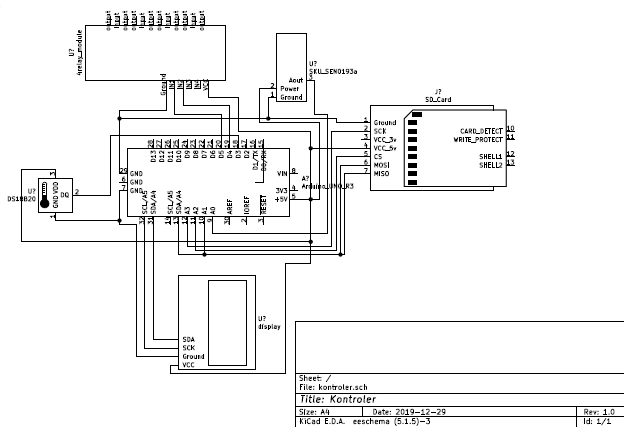
\includegraphics[width=\textwidth]{kontroler.png}

Ulaze i izlaze modula kačimo direktno na kontroler. Na relej se kači svetlo, pumpa za vodu i ventilatori(na jedan terminal kačimo 9V, a na drugi 12V).

\section{Softverski dizajn}

\subsection{Pokretanje i princip rada}

U inicijalnom setup petlji kontrolera inicijalizujemo sve potrebne biblioteke i promenljive. 

Glavna petlja ce pratiti sledeći sablon rada:

\hrulefill
\begin{itemize}
  \item Hvatanje temperature,
  \item hvatanje vlage zemlje,
  \item pokretanje pomoćne funckije koja odredjuje akcije u vidu zalivanja ili regulacije toplote,
  \item zapisivanje podataka i akcija,
  \item ispis na ekran.
\end{itemize}
\hrulefill

\subsection{Temperatura}

Hvatanje temperature vrsi se pozivom funkcije \verb|read_temperature()| koja će od senzora zatražiti trenutnu temperaturu. Ako je doslo do greske vratiće staru vrednost u protivnom biće vraćena očitana. 

\begin{lstlisting}
  /*
  * Funkcija za citanje temperature preko senzora
  * @return float - temp
  */
 float read_temperature(){
   // Var za temperaturu
   float tempC = sensors.getTempCByIndex(0);
   
   // Trazimo temperaturu
   Serial.print("Hvatam temperaturu");
   sensors.requestTemperatures();
   Serial.println("uspeh");
 
   Serial.print("Temperatura za device 1 (index 0) je: ");
   Serial.println(tempC);
 
   if(tempC != DEVICE_DISCONNECTED_C) return tempC;
 
   // Exception
   else Serial.println("Greska prilikom citanja!");
   return null;
 }
\end{lstlisting}
  
\subsection{Vlaga zemlje}

Što se vlage zemlje tiče proces je isti, funkcija izgleda ovako:

\begin{lstlisting}
  /*
 * Funkcija za citanje vlage zemlje preko senzora
 * @return float - soil_val
 */
float read_soil_moisture(){

	Serial.print("Hvatam vlagu");

	// Citanje vlaznosti
	int soil_val = analogRead(SENSOR_PIN);

	// Konverzija
	soil_val = map(soil_val, 550, 0, 0, 100);

	Serial.print("Vlaga: ");
	Serial.print(soil_val);

	return soil_val;
}
  \end{lstlisting}

  \subsection{Obrada učitanih vrednosti}

  Obrada vrednosti vrši se pozivom funkcije \verb|process_inputs|

  \begin{lstlisting}
    /*
    * Funkcija za kontrolu toka i logovanja
    * @param temp_val - temperatura
    * @param soil_val - vlaga
    */
   void process_inputs(float temp_val, float soil_val){
    
     // Aktivacija pumpe
     if(soil_val < SOIL_MOISTURE_TRESHOLD) digitalWrite(relay4, LOW);

     // Palimo 12V
     if(temp_val>= 30){
      digitalWrite(relay1, HIGH);
      digitalWrite(relay2, LOW);
     }

     // Gasimo oba
     if(temp_val<=20){
       digitalWrite(relay1, HIGH);
       digitalWrite(relay2, HIGH);
     }

     // Palimo 9V
     else{
       digitalWrite(relay1, HIGH);
       digitalWrite(relay2, LOW);
     }
   }
    \end{lstlisting}

  
    \subsection{Ispis na ekran}

    Ova funkcija prvo konvertuje vrednosti u stringove i smešta ih u char niz. Nakon što su smešteni u svoje bafere pozivaju se funkcije za ispis.

    
  \begin{lstlisting}
    /*
     * Funkcija za ispis na ekran
     * @param temp_val - temperatura
     * @param soil_val - vlaga
     */
    void output_values(float temp_val, float soil_val){

	  //Pravimo char array za drawStr funkciju
	  String temp_string = String(temp_val);
	  String soil_string = String(soil_val);

	  char temp_buffer[5];
	  temp_string.toCharArray(temp_buffer, 5);

	  char soil_buffer[5];
	  soil_string.toCharArray(soil_buffer, 5);

	  //Ispis na ekran
	  temp_out(temp_buffer);
	  delay(2000);
	  soil_out(soil_buffer);  
  }
    \end{lstlisting}


\chapter{Izgradnja modela}

Kada smo definisali plan sistema možemo započeti izradu modela. Za početak odredjujemo tok operacija koje naš sistem treba da izvrši. Imajući na umu da modelujemo kontroler sistema, možemo ga posmatrati kao automat. Po definicija automata, mi modelujemo prelaze stanja koji su elementi nekog konačnog skupa stanja Q. Stoga, osnovni tok operacija se može predstaviti flowchart-om koji izgleda ovako:

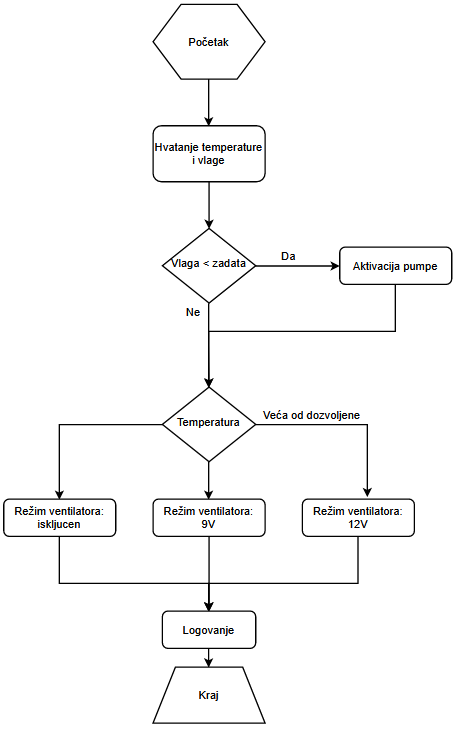
\includegraphics[width=\textwidth]{flow.png}

Ovim smo predstavili jedan ciklus sistema koji se izvršava kontinualno. Sada možemo izraditi koncept modela.


\section{Konceptualizacija modela}

Kako bismo stvorili koncept modela moramo se vratiti na funkcije našeg sistema. Analizom funkcija i konkretnog hardvera pronalazimo uslove i ograničenja sistema koji modelujemo. Mi smo ranije u radu prešli rad odredjenih komponenti koje su od značaja za rad sistema, sada odredjujemo njihovu korelaciju unutar sistema. Ako pogledamo sliku PID kontrolera:

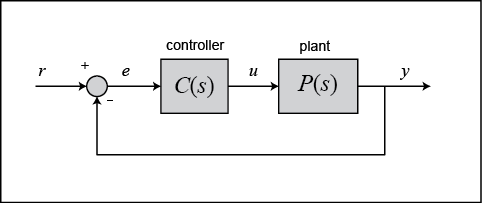
\includegraphics[width=\textwidth]{feedback_block.png}

zaključicemo da je naš sistem idealan primer istog.

Sa leve strane imamo promenljivu $r$ koja predstavlja idealan output sistema. Naš model će se fokusirati na regulaciju temperature stoga mi želimo da nam $r$ bude vrednost unutar opsega 20-30$^\circ$C. Uzećemo 25$^\circ$C kao fiksnu vrednost. 

$Plant$ ili $P(s)$ nam predstavlja sistem koji želimo kontrolisati. Možemo primetiti da on ima ulaznu vrednost($u$) koja nam utiče na izlaz $y$. Da bi sistem izvrsio validaciju on će izlazni signal da uporedi sa zadatom vrednosti. Rezultat te operacije($e$) se prosledjuje kao input kontroleru $C(s)$ koji onda na osnovu njega utiče na sistem. U našem slučaju sistem će izgledati ovako:\\

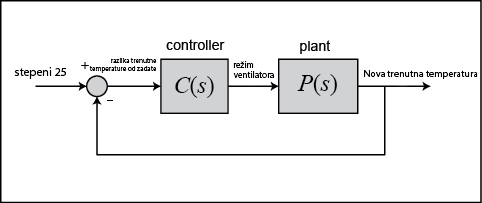
\includegraphics[width=\textwidth]{feedback.png}



\section{Kolekcija podataka}

Podatke možemo prikupiti preko samih proizvodjača komponenti za koje smo se opredelili. Čitanjem tehničke dokumentacije ili samih specifikacija proizvoda možemo stvoriti gruba očekivanja kako će se sistem ponašati u realnim uslovima. \\

\noindent Bitno je imati na umu da vredonosti koje nam proizvodjač da uglavnom nisu merodavne pa je neophodno, ukoliko je to moguće, istraživanjem utvrditi realne performanse komponente. Ukoliko nije moguće naći iste, kako bi izbegli dodatne troskove, moramo uračunati do 30\% devijacije od datih. U ovom radu, prilikom planiranja mi smo izvršili kolekciju i obradu podataka da bi stvori plan stoga nam preostaje prevodjenje modela i izrada simulacije. Jedino sto nam preostaje jeste sistem za zalivanje koji ne utiče direktno na ambijent mašine, njega ćemo posebno simulirati putem takozvanog pilotnog projekta. 


\subsection{Regulacija zalivanja - pilotni projekat}

Za projekat sam pronašao saksiju adekvatnih veličina za sistem. Saksija je napunjana sa $2/3$ zemlje i $1/3$ perlita čija je uloga da pomogne oko drenaže(ako za to bude potrebe). Do saksije je sprovedeno crevo po obodu sa sitnim rupicama za zalivanje. Sada preostaje razmatranje pumpe:

Budući da je naš sistem relativno malih razmera koji podrzava jednu biljku neće nam biti potrebna velika pumpa. Ako se okrenemo akvaristici možemo pronaći sasvim idealnu pumpu za projekat. 
Zalivanje vrši se putem pumpe za manje akvarijume. Po specifikaciji proizvodjača protok vode iznosi $Q = 150 l/h$. Testiranjem je utvrdjeno sledeće:

\begin{table}[ht]
  \caption{Rad pumpe za vodu}
  \centering
  \begin{tabular}{|c|c|}
  \hline
    Trajanje[sekunde] & Količina vode u posudi[$l$]\\ \hline
  0 & 0 \\ \hline
  15 & 0.5 \\ \hline
  30 & 1.2 \\ \hline
  60 & 2.4 \\ \hline
  \end{tabular}
\end{table}

Testiranjem je utvrdjena tačnost specifikacije i sada nam ostaje da odredimo dužinu vremenskog perioda za koji će relej držati pumpu otvorenom.

Saksija koju ćemo koristiti ovde iznosi $1.5l$ što znači da ako pogledamo tabelu, možemo uočiti da je $~10s$ sasvim dovoljno da se potopi zemlja unutar saksije.

Ovo nije optimalna količina vode ali nam pruža sigurnost od prelivanja. Pumpa će se aktivirati opet ukoliko vlažnost zemlje ne odgovara našem standardu.

\section{Prevodjenje modela}

\section{Verifikacija}
 
\section{Validacija}

\chapter{Izvršavanje simulacije}

\section{Dizajn eksperimenta}

\section{Izvršavanje i analiza}

\section{Dodatna izvršavanja}

\chapter{Implementacija}

\section{Dokumentacija i izveštaj}

\chapter{Izvori}

www.agropress.org - http://www.agropress.org.rs/lat/rubrike/biljna-proizvodnja/ratarstvo-i-povrtarstvo/item/1713-koje-su-prednosti-plastenicke-proizvodnje

\end{document}

%\section*{Acknowledgements}
%\begin{itemize}
%\item A special word of thanks goes to Professor Don Knuth\footnote{\url{http://www-cs-faculty.stanford.edu/~uno/}} (for \TeX{}) and Leslie Lamport\footnote{\url{http://www.lamport.org/}} (for \LaTeX{}).
%\item I'll also like to thank Gummi\footnote{\url{http://gummi.midnightcoding.org/}} developers and LaTeXila\footnote{\url{http://projects.gnome.org/latexila/}} development team for their awesome \LaTeX{} editors.
%\item I'm deeply indebted my parents, colleagues and friends for their support and encouragement.
%\end{itemize}

%%%%%%%%%%%%%%%%%%%%%%%%%%%%%%%%%%%%%%%%%%%%%%%%%%%%%%%
% Sample table                                        %
% Source: www1.maths.leeds.ac.uk/latex/TableHelp1.pdf %
%%%%%%%%%%%%%%%%%%%%%%%%%%%%%%%%%%%%%%%%%%%%%%%%%%%%%%%
%\begin{table}[ht]
 % \caption{Sample table} % title of Table
  %\centering % used for centering table
  %\begin{tabular}{c c c c}
  % centered columns (4 columns)
  %\hline\hline %inserts double horizontal lines
  %S. No. & Column\#1 & Column\#2 & Column\#3 \\ [0.5ex]
  % inserts table
  %heading
  %\hline % inserts single horizontal line
  %1 & 50 & 837 & 970 \\
  %2 & 47 & 877 & 230 \\
  %3 & 31 & 25 & 415 \\
  % & 35 & 144 & 2356 \\
  %5 & 45 & 300 & 556 \\ [1ex] % [1ex] adds vertical space
  %\hline %inserts single line
  %\end{tabular}
  %\label{table:nonlin} % is used to refer this table in the text
  %\end{table}